%%%%%%%%%%%%%%%%%%%%%%%%%%%%%%%%%%%%%%%%%
% Beamer Presentation
% LaTeX Template
% Version 1.0 (10/11/12)
%
% This template has been downloaded from:
% http://www.LaTeXTemplates.com
%
% License:
% CC BY-NC-SA 3.0 (http://creativecommons.org/licenses/by-nc-sa/3.0/)
%
%%%%%%%%%%%%%%%%%%%%%%%%%%%%%%%%%%%%%%%%%

%----------------------------------------------------------------------------------------
%	PACKAGES AND THEMES
%----------------------------------------------------------------------------------------

\documentclass{beamer}
\usepackage{biblatex} % Utilisation du package biblatex
\addbibresource{references.bib} % Chargement du fichier .bib

\mode<presentation> {

% The Beamer class comes with a number of default slide themes
% which change the colors and layouts of slides. Below this is a list
% of all the themes, uncomment each in turn to see what they look like.

%\usetheme{default}
%\usetheme{AnnArbor}
%\usetheme{Antibes}
%\usetheme{Bergen}
%\usetheme{Berkeley}
%\usetheme{Berlin}
%\usetheme{Boadilla}
%\usetheme{CambridgeUS}
%\usetheme{Copenhagen}
%\usetheme{Darmstadt}
%\usetheme{Dresden}
%\usetheme{Frankfurt}
%\usetheme{Goettingen}
%\usetheme{Hannover}
%\usetheme{Ilmenau}
%\usetheme{JuanLesPins}
%\usetheme{Luebeck}
\usetheme{Berlin}
%\usetheme{Malmoe}
%\usetheme{Marburg}
%\usetheme{Montpellier}
%\usetheme{PaloAlto}
%\usetheme{Pittsburgh}
%\usetheme{Rochester}
%\usetheme{Singapore}
%\usetheme{Szeged}
%\usetheme{Warsaw}

% As well as themes, the Beamer class has a number of color themes
% for any slide theme. Uncomment each of these in turn to see how it
% changes the colors of your current slide theme.

%\usecolortheme{albatross}
%\usecolortheme{beaver}
%\usecolortheme{beetle}
%\usecolortheme{crane}
%\usecolortheme{dolphin}
%\usecolortheme{dove}
%\usecolortheme{fly}
%\usecolortheme{lily}
%\usecolortheme{orchid}
%\usecolortheme{rose}
%\usecolortheme{seagull}
%\usecolortheme{seahorse}
%\usecolortheme{whale}
%\usecolortheme{wolverine}

%\setbeamertemplate{footline} % To remove the footer line in all slides uncomment this line

% Commande pour la footline personnalisée
\makeatletter
\defbeamertemplate*{footline}{custom theme}
{
  \leavevmode%
  \hbox{%
  \begin{beamercolorbox}[wd=.15\paperwidth,ht=2.5ex,dp=1.0ex,leftskip=1em]{author in head/foot}%
    \usebeamerfont{author in head/foot}\insertshortauthor
  \end{beamercolorbox}%
  \begin{beamercolorbox}[wd=.15\paperwidth,ht=2.5ex,dp=1.0ex,center]{author in head/foot}%
    \usebeamerfont{title in head/foot}\insertshortinstitute
  \end{beamercolorbox}%
  \begin{beamercolorbox}[wd=.5\paperwidth,ht=2.5ex,dp=1.0ex,center]{title in head/foot}%
    \usebeamerfont{title in head/foot}\insertshorttitle
  \end{beamercolorbox}%
  \begin{beamercolorbox}[wd=.2\paperwidth,ht=2.5ex,dp=1.0ex,rightskip=1em]{title in head/foot}%
    \usebeamerfont{title in head/foot}\hfill\insertframenumber/\inserttotalframenumber
  \end{beamercolorbox}}%
  \vskip0pt%
}
\makeatother
\setbeamertemplate{headline}{}
\setbeamertemplate{navigation symbols}{} % To remove the navigation symbols from the bottom of all slides uncomment this line
}
\usepackage{subfigure}
\usepackage{tikz}
\usetikzlibrary{arrows, automata}
\tikzset{every picture/.style={scale=1,auto=center,every node/.style={circle, draw=black!50,fill=blue!20}}}
\usepackage{forest}
\usepackage{graphicx} % Allows including images
\usepackage{booktabs} % Allows the use of \toprule, \midrule and \bottomrule in tables
\usepackage{multicol}
\usepackage{algorithm}
\usepackage{algpseudocode}
\usepackage{listings}
\usepackage{listings-rust}
\definecolor{codegreen}{rgb}{0,0.6,0}
\definecolor{codegray}{rgb}{0.5,0.5,0.5}
\definecolor{codepurple}{rgb}{0.58,0,0.82}
\definecolor{backcolour}{rgb}{0.95,0.95,0.92}

\lstdefinestyle{mystyle}{
    backgroundcolor=\color{backcolour},
    commentstyle=\color{codegreen},
    keywordstyle=\color{magenta},
    numberstyle=\tiny\color{blue},
    stringstyle=\color{codepurple},
    basicstyle=\tiny,
    breakatwhitespace=false,
    breaklines=true,
    captionpos=b,
    keepspaces=true,
    numbers=left,
    numbersep=5pt,
    showspaces=false,
    showstringspaces=false,
    showtabs=false,
    tabsize=2
}

\lstset{style=mystyle}
%----------------------------------------------------------------------------------------
%TITLE PAGE
%----------------------------------------------------------------------------------------

\title[Énumération des cliques maximales]{Étude comparative d'algorithmes d'énumération des cliques maximales d'un graphe simple} % The short title appears at the bottom of every slide, the full title is only on the title page

\author{Virgil Surin} % Your name
\institute[UMONS] % Your institution as it will appear on the bottom of every slide, may be shorthand to save space
{
Université de Mons \\ % Your institution for the title page
\medskip
Directeur: \textit{Hadrien Mélot} % Your email address
}
\date{\today} % Date, can be changed to a custom date

\begin{document}

\begin{frame}
\titlepage % Print the title page as the first slide
\end{frame}

\begin{frame}
\frametitle{Table des matières} % Table of contents slide, comment this block out to remove it
\tableofcontents % Throughout your presentation, if you choose to use \section{} and \subsection{} commands, these will automatically be printed on this slide as an overview of your presentation
\end{frame}

%----------------------------------------------------------------------------------------
%	PRESENTATION SLIDES
%----------------------------------------------------------------------------------------

%------------------------------------------------
\section{Introduction}
\begin{frame}
\frametitle{Introduction}
\begin{block}{Motivation}
  L'énumération des cliques maximales dans un graphe simple est un problème coûteux en temps avec de nombreuses applications concrètes (biologie, sociologie, informatique, etc.).
\end{block}
\pause
\begin{block}{Objectif}
  L'objectif de ce projet était d'étudier plusieurs algorithmes d'énumération de cliques maximales dans un graphe simple non orienté et de comparer leurs performances.
  \begin{itemize}
    \item Basé sur un article de Conte et Tomita\cite{CONTE20221}
    \item Implémentation en \emph{Python} de 4 algorithmes
    \item Comparaison des performances des algorithmes
    \item Implémentation en \emph{Rust} et comparaison avec \emph{Python}
  \end{itemize}
\end{block}
\end{frame}

%------------------------------------------------
\section{Notions théoriques}

\subsection{Graphes}
\begin{frame}
\frametitle{Les graphes simples}
\begin{definition}
  Un graphe simple non orienté est défini par un ensemble de nœuds \(V\) et un ensemble d'arêtes \(E\). Chaque arête relie une paire de nœuds distincts sans direction associée, ce qui signifie que l'arête \((v, w)\) est identique à l'arête \((w, v)\).
\end{definition}
\begin{example}
  \begin{columns}
    \column{0.38\textwidth}
    Graphe avec 4 nœuds :\vspace*{0.4cm}
    \(V = \{1,2,3,4\}\)\\
    $E = \{(1,2), (1, 3), (2,3), (3,4)\}$
    \column{0.38\textwidth}
    \begin{figure}
      \centering
      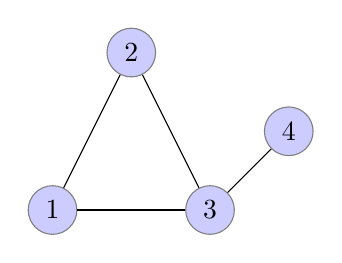
\begin{tikzpicture}

        \node (n1) at (0, 0) {1};
        \node (n2) at (1, 2) {2};
        \node (n3) at (2, 0) {3};
        \node (n4) at (3, 1) {4};

        \foreach \from/\to in {n1/n2, n2/n3, n1/n3, n3/n4}
        \draw (\from) -- (\to);
      \end{tikzpicture}
    \end{figure}
  \end{columns}
\end{example}
\end{frame}

\subsection{Cliques}
\begin{frame}
  \frametitle{Cliques maximales}
  \begin{definition}
    Une clique dans un graphe est un sous-ensemble de nœuds tel que chaque paire de nœuds est connectée par une arête.
  \end{definition}
  \begin{definition}
    Une clique est dite maximale si aucun nœud supplémentaire ne peut être ajouté sans perdre la propriété de clique. Une clique maximale est donc un sous-graphe complet qui ne peut être étendu.
  \end{definition}
  \begin{example}
    \begin{columns}
      \column{0.38\textwidth}
      Le graphe suivant possède les cliques maximales suivantes :
      \begin{itemize}
        \item \{1, 2, 3\}
        \item \{3, 4\}
      \end{itemize}
      \column{0.38\textwidth}
      \begin{figure}
        \centering
        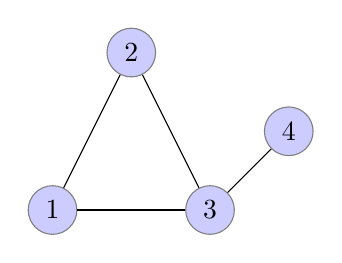
\begin{tikzpicture}

          \node (n1) at (0, 0) {1};
          \node (n2) at (1, 2) {2};
          \node (n3) at (2, 0) {3};
          \node (n4) at (3, 1) {4};

          \foreach \from/\to in {n1/n2, n2/n3, n1/n3, n3/n4}
          \draw (\from) -- (\to);
        \end{tikzpicture}
      \end{figure}
    \end{columns}
  \end{example}
\end{frame}

%------------------------------------------------
\section{Les algorithmes}
\subsection{Structure générale}%
\label{subsec:struct}

\begin{frame}
  \frametitle{Structure générale}
  \begin{center}
  \scalebox{0.70}{
    \begin{minipage}{1\linewidth}
      \begin{algorithm}[H]
        \textbf{Input}: un graphe $G = (V,E)$

        \textbf{Output}: toutes les cliques maximales de $G$
        \begin{algorithmic}[1]
          \Procedure{ALG}{$SUBG, CAND$}
          \If{$SUBG = \emptyset$} \Comment{$Q$ est une clique maximale}
          \State \textbf{print} ($ Q $)
          \Else
          \State $u \gets$ un nœud pivot de \emph{SUBG}
          \While{il reste des nœuds candidats}
          \State $p \gets$ un nœud dans $CAND \setminus N(u)$
          \State $ Q \cup p $ \Comment{on ajoute \emph{p} à $Q$}
          \State // Mise à jour des paramètres
          \State $SUBG_p \gets SUBG \cap N(p)$
          \State $CAND_p \gets CAND \cap N(p)$
          \State \Call{ALG}{$SUBG_p, CAND_p$}
          \State $CAND \gets CAND \setminus {p}$
          \State $ Q \setminus p $ \Comment{on retire \emph{p} de $Q$}
          \EndWhile
          \EndIf
          \EndProcedure
          \State \Call{ALG}{$V,V$}
        \end{algorithmic}
        \caption{Squelette de base}
        \label{fig:alg}
      \end{algorithm}
    \end{minipage}
  }
  \end{center}
\end{frame}

\subsection{Bron-Kerbosch}
\begin{frame}
\frametitle{Algorithme de Bron-Kerbosch}
L'algorithme de Bron-Kerbosch est une méthode récursive pour énumérer toutes les cliques maximales dans un graphe. Il existe plusieurs variantes de cet algorithme :
\begin{itemize}
    \item \textbf{Sans pivot :} Cette version explore toutes les combinaisons possibles de nœuds sans aucune optimisation particulière. Elle itère sur tous les candidats possibles pour construire les cliques maximales.
  \item \textbf{Avec pivot aléatoire :} Un nœud pivot est choisi aléatoirement parmi les nœuds disponibles.
  \item \textbf{Avec pivot de degré maximum :} Ici, le pivot est choisi comme étant le nœud ayant le plus grand nombre de voisins, ce qui permet de réduire davantage les appels récursifs en élaguant la recherche.
\end{itemize}
La complexité temporelle de ces variantes dans le pire des cas est \(O(3^{n/3})\), correspondant au nombre maximum de cliques maximales dans un graphe.
\end{frame}

\subsection{CLIQUES}
\begin{frame}
\frametitle{Algorithme CLIQUES}
L'algorithme CLIQUES est une optimisation de Bron-Kerbosch qui sélectionne un pivot de manière à minimiser le nombre de récursions nécessaires. Ce pivot est choisi pour maximiser l'intersection entre les candidats et les voisins du pivot, c'est-à-dire \(CAND \cap N(u)\).

CLIQUES est la variante de Bron-Kerbosch dont on attend les meilleures performances.
\end{frame}

\begin{frame}
  \frametitle{Bref exemple}
  \begin{columns}
    \column{0.28\textwidth}
    \begin{figure}
      \centering
      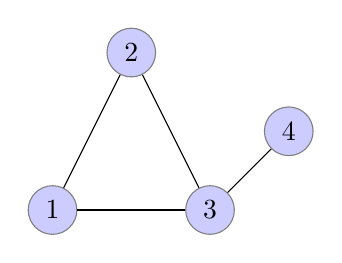
\begin{tikzpicture}

        \node (n1) at (0, 0) {1};
        \node (n2) at (1, 2) {2};
        \node (n3) at (2, 0) {3};
        \node (n4) at (3, 1) {4};

        \foreach \from/\to in {n1/n2, n2/n3, n1/n3, n3/n4}
        \draw (\from) -- (\to);
      \end{tikzpicture}
    \end{figure}
    \column{0.70\textwidth}
    \begin{figure}[ht]
      \centering
      \forestset{
        mynode/.style={
          for tree={
            rectangle, draw, text centered, align=left, anchor=north,
            edge={-latex},
            parent anchor=south, child anchor=north,
            l sep+=1cm, % increase level separation
            s sep+=0.5cm, % increase sibling separation
            inner xsep=7pt, % horizontal padding
            inner ysep=3pt, % vertical padding
            font=\normalsize,
            scale=0.3,
          }
        },
        EL/.style = {
          edge label={node[rectangle, midway, fill=white, draw=none, anchor=center, font=\tiny]{#1}}
        }
      }
      \begin{forest}
        mynode
        [{SUBG = \{1, 2, 3, 4\}\\
          CAND = \{1, 2, 3, 4\}\\
          u = 3\\
          CAND - N(u) = \{3\}}
        [{SUBG = \{1, 2, 4\}\\
          CAND = \{1, 2, 4\}\\
          u = 1\\
          CAND - N(u) = \{1, 4\}}, EL={p=3}
        [{SUBG = \{2\}\\
          CAND = \{2\}\\
          u = 2\\
          CAND - N(u) = \{2\}}, EL={p=1}
        [{SUBG = \{\}\\
          CAND = \{\}\\
          Clique: \{3, 1, 2\}}, EL={p=2}]
        ]
        [{SUBG = \{\}\\
          CAND = \{\}\\
          Clique: \{3, 4\}}, EL={p=4}]
        ]
        ]
      \end{forest}
    \end{figure}
  \end{columns}
\end{frame}

% ------------------------------------------------
\section{Résultats}
\begin{frame}
  \frametitle{Test sets}
  \begin{block}{Premier ensemble de test}
    Ensemble des graphes d'ordre 4 à 10 inclus. (Soit 12 278 357 graphes)
  \end{block}
  \begin{block}{Deuxième ensemble de test}
    3 types de graphes différents, d'ordre 3 à 45 sélectionnés pour leurs propriétés spécifiques:
    \begin{itemize}
      \item Graphe vide (autant de cliques maximales que de nœuds)
      \item Graphe complet (une seule clique maximale contenant tous les nœuds)
      \item Graphe de Moon-Moser (contient le nombre maximum de cliques maximales possible, soit \(3^{n/3}\), où \emph{n} est le nombre de nœuds)
    \end{itemize}
  \end{block}
\end{frame}

\subsection{Python}
\begin{frame}
  \frametitle{Résultats en Python - Premier test set}
  \begin{columns}
    \column{0.48\textwidth}
      \centering
      \includegraphics[width=\textwidth]{images/total_plot.png}
      \caption{Temps total moyen pour énumérer toutes les cliques maximales}
    \column{0.48\textwidth}
      \centering
      \includegraphics[width=\textwidth]{images/delay_plot.png}
      \caption{Délai moyen pour énumérer une clique maximale}
  \end{columns}
\end{frame}

\begin{frame}
  \frametitle{Résultats en Python - Second test set}
  \begin{columns}
    \column{0.32\textwidth}
    \centering
    \includegraphics[width=\textwidth]{images/total_pivot_empty_plot.png}
    \caption{Graphes vides}
    \column{0.32\textwidth}
    \centering
    \includegraphics[width=\textwidth]{images/total_pivot_turan_plot.png}
    \caption{Moon-Moser}
    \column{0.32\textwidth}
    \centering
    \includegraphics[width=\textwidth]{images/total_pivot_complete_plot.png}
    \caption{Graphes complets}
  \end{columns}
  \begin{center}
    Temps totaux moyens
  \end{center}
  \begin{columns}
    \column{0.32\textwidth}
    \centering
    \includegraphics[width=\textwidth]{images/delay_pivot_empty_plot.png}
    \caption{Graphes vides}
    \column{0.32\textwidth}
    \centering
    \includegraphics[width=\textwidth]{images/delay_pivot_turan_plot.png}
    \caption{Moon-Moser}
    \column{0.32\textwidth}
    \centering
    \includegraphics[width=\textwidth]{images/delay_pivot_complete_plot.png}
    \caption{Graphes complets}
  \end{columns}
  \begin{center}
    Délais moyens
  \end{center}
\end{frame}

\begin{frame}
\frametitle{Résultats en Python - Conclusion}
\begin{block}{Conclusion}
\begin{itemize}
  \item Courbes exponentielles peu importe l'algorithme (se voit surtout sur les graphes de Moon-Moser)
  \item Le délai est bien linéaire
  \item Certains algorithmes sont meilleurs selon le type de graphe (exemple : CLIQUES ne performe pas bien sur les graphes complets)
\end{itemize}
\end{block}
\end{frame}

\subsection{Comparaison entre Python et Rust}
\begin{frame}
\frametitle{Comparaison Python vs Rust - Premier test set}
\begin{columns}
  \column{0.24\textwidth}
  \centering
 \includegraphics[width=\textwidth]{images/total_new_pyrust_CLIQUES_plot.png}
  \caption{CLIQUES}%
  \column{0.24\textwidth}
  \centering
  \includegraphics[width=\textwidth]{images/total_new_pyrust_BK_plot.png}
  \caption{Bron-Kerbosch}%
  \column{0.24\textwidth}
  \centering
  \includegraphics[width=\textwidth]{images/total_new_pyrust_BKP_M_plot.png}
  \caption{BKP\_M}%
  \column{0.24\textwidth}
  \centering
  \includegraphics[width=\textwidth]{images/total_new_pyrust_BKP_R_plot.png}
  \caption{BKP\_R}%
  \end{columns}
  \begin{center}
    Temps totaux moyens
  \end{center}
\end{frame}

\begin{frame}
\frametitle{Comparaison Python vs Rust - Second test set}
CLIQUES
  \begin{columns}
    \column{0.32\textwidth}
    \centering
    \includegraphics[width=\textwidth]{images/total_CLIQUES_new_pyrust_pivot_empty_plot.png}
    \caption{Graphes vides}
    \column{0.32\textwidth}
    \centering
    \includegraphics[width=\textwidth]{images/total_CLIQUES_new_pyrust_pivot_turan_plot.png}
    \caption{Moon-Moser}
    \column{0.32\textwidth}
    \centering
    \includegraphics[width=\textwidth]{images/total_CLIQUES_new_pyrust_pivot_complete_plot.png}
    \caption{Graphes complets}
  \end{columns}
  \begin{center}
    Temps totaux moyens
  \end{center}
\end{frame}

\begin{frame}
\frametitle{Comparaison Python vs Rust - Second test set}
Bron-Kerbosch avec pivot de degré maximum
  \begin{columns}
    \column{0.32\textwidth}
    \centering
    \includegraphics[width=\textwidth]{images/total_BKP_M_new_pyrust_pivot_empty_plot.png}
    \caption{Graphes vides}
    \column{0.32\textwidth}
    \centering
    \includegraphics[width=\textwidth]{images/total_BKP_M_new_pyrust_pivot_turan_plot.png}
    \caption{Moon-Moser}
    \column{0.32\textwidth}
    \centering
    \includegraphics[width=\textwidth]{images/total_BKP_M_new_pyrust_pivot_complete_plot.png}
    \caption{Graphes complets}
  \end{columns}
  \begin{center}
    Temps totaux moyens
  \end{center}
\end{frame}

\begin{frame}
\frametitle{Comparaison Python vs Rust - Second test set}
Bron-Kerbosch avec pivot aléatoire
  \begin{columns}
    \column{0.32\textwidth}
    \centering
    \includegraphics[width=\textwidth]{images/total_BKP_R_new_pyrust_pivot_empty_plot.png}
    \caption{Graphes vides}
    \column{0.32\textwidth}
    \centering
    \includegraphics[width=\textwidth]{images/total_BKP_R_new_pyrust_pivot_turan_plot.png}
    \caption{Moon-Moser}
    \column{0.32\textwidth}
    \centering
    \includegraphics[width=\textwidth]{images/total_BKP_R_new_pyrust_pivot_complete_plot.png}
    \caption{Graphes complets}
  \end{columns}
  \begin{center}
    Temps totaux moyens
  \end{center}
\end{frame}

\begin{frame}[fragile]
  \frametitle{Comparaison Python vs Rust}
  \begin{columns}
\column{0.48\textwidth}
  \begin{figure}[h]
  \begin{lstlisting}[language=Rust]
        let subg_vec: Vec<&u32> = subg.iter().collect();
        let u = subg_vec.choose(&mut rng).unwrap();
        let u_neighbors: HashSet<_> = g.adj[&u].iter().copied().collect();
        for p in cand.difference(&u_neighbors).copied().collect::<Vec<u32>>() {
            let p_neighbors: HashSet<_> = g.adj[&p].iter().copied().collect();
  \end{lstlisting}
  \caption{Extrait de code Rust}
  \end{figure}
\column{0.48\textwidth}
  \begin{figure}[h]
  \begin{lstlisting}[language=Python]
        u = random.choice(list(SUBG))
        for p in CAND - G.adj[u]:
            p_neighbors = G.adj[p]
  \end{lstlisting}
  \caption{Extrait de code Python}
  \end{figure}
  \end{columns}
\end{frame}

\begin{frame}
\frametitle{Comparaison Python vs Rust - Conclusion}
\begin{block}{Conclusion}
\begin{itemize}
  \item Rust est bien meilleur que Python de manière générale
  \item Résultats clairement inférieurs ou mitigés sur des graphes spéciaux, probablement à cause de l'implémentation (\emph{HashSet})
\end{itemize}
\end{block}
\end{frame}
%------------------------------------------------
\section{Conclusion}
\begin{frame}
\frametitle{Conclusion}
\begin{block}{Conclusion}
  \begin{itemize}
    \item Les algorithmes de Bron-Kerbosch avec pivot et CLIQUES sont très efficaces
    \item Les algorithmes sont sensibles au type de graphe
    \item Le choix du pivot est important (coût en performance)
    \item Moyennant une bonne implémentation, on peut obtenir des gains significatifs en Rust par rapport à Python
  \end{itemize}
\end{block}
\end{frame}

\begin{frame}
\frametitle{Questions}
Merci pour votre attention. Des questions ?
\end{frame}

%------------------------------------------------
\section{Bibliographie}
\begin{frame}[allowframebreaks]
\frametitle{Bibliographie}
\printbibliography
\end{frame}


\end{document}
